\section{Iteration 3}
\label{i3}
Wie bereits nach der ersten Iteration wurde dem Auftraggeber auch nach der zweiten Iteration
anhand einer kurzen Demonstration der Entwicklungsstand präsentiert.

Folgende Punkte sind dabei rückgemeldet worden:
\begin{itemize}
    \item Die für Desktops optimiert Benutzerschnittstelle entspricht den Vorstellungen und wirkt intuitiv.
    \item Da vom Auftraggeber keine echten \ac{THD}-Werte zur Verfügung gestellt werden können,
          können diese weggelassen werden.
    \item Die Applikation soll um den in der Aufgabenstellung (Anhang \ref{anhang:aufgabenstellung}) beschrieben Use Case:
          ``Eine benutzerdefinierte Zeitspanne der Messwerte mittels vorgegebener
          Labels beschriften. Bsp.: («Backofen war von 09:31 – 10:15 aktiv»)`` erweitert werden.
    \item Die Übertragung der Messdaten mittels \ac{MQTT} soll,
          wie bereits in der Aufgabenstellung (Anhang \ref{anhang:aufgabenstellung}) verlangt, mit \ac{TLS} verschlüsselt werden.
\end{itemize}
In der letzten der drei Iterationen wurden diese finalen Anforderungen umgesetzt.
Die nächsten Abschnitte berichten darüber.

\subsection{Labeling}
Wie in Kapitel \ref{cap1} beschrieben, ist ein Ziel dieser Arbeit,
dass Messdaten für Supervised Learning aufbereitet werden können.
Dazu müssen diese mit Labels versehen werden.
Was grundsätzlich unter Labels zu verstehen ist, wird im Abschnitt \ref{state:supervised-learning} Supervised Learning erklärt.
\begin{figure}
    \centering
    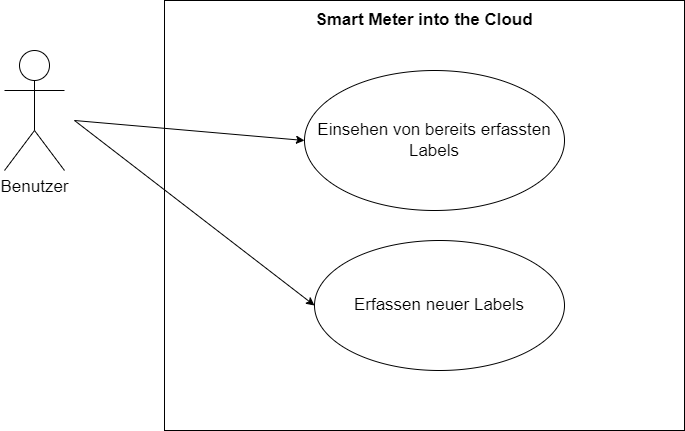
\includegraphics[width=1.0\textwidth]{gfx/labeling.drawio}
    \caption{Anwendungsfall Diagramm zu Labeling}
    \label{fig:labeling}
\end{figure}
Für diese Arbeit sollen Zeitabschnitte, während denen Messdaten erfasst wurden, mit Labels versehen werden.
Ein Label entspricht dabei einem Typ von Stromverbraucher wie beispielsweise einem Backofen oder einem Kühlschrank.

Die beiden dazugehörigen Anwendungsfälle sind in Abbildung \ref{fig:labeling} dargestellt.
Um diese zu implementieren,
mussten Anpassungen an der Benutzerschnittstelle sowie an der \ac{API} vorgenommen werden.

\subsubsection{Benutzerschnittstelle}
Um das Erfassen von Labels intuitiv zu gestalten,
wurden die Graphen so angepasst, dass mit der Maus per Drag ein Zeitabschnitt markiert werden kann.
Die in Abbildung \ref{fig:add_label} gezeigte Komponente `New Label` wird dann angezeigt, wenn ein Zeitabschnitt angewählt wurde.
Sie beinhaltet genaue Angaben zum ausgewählten Abschnitt
und ermöglicht es, das passende Label auszuwählen. \footnote{
    In der Abbildung dienen `Label one` und `Label two` als Platzhalter für richtige Labels wie beispielsweise `Kühlschrank` oder `Waschmaschine`}.

\begin{figure}[H]
    \centering
    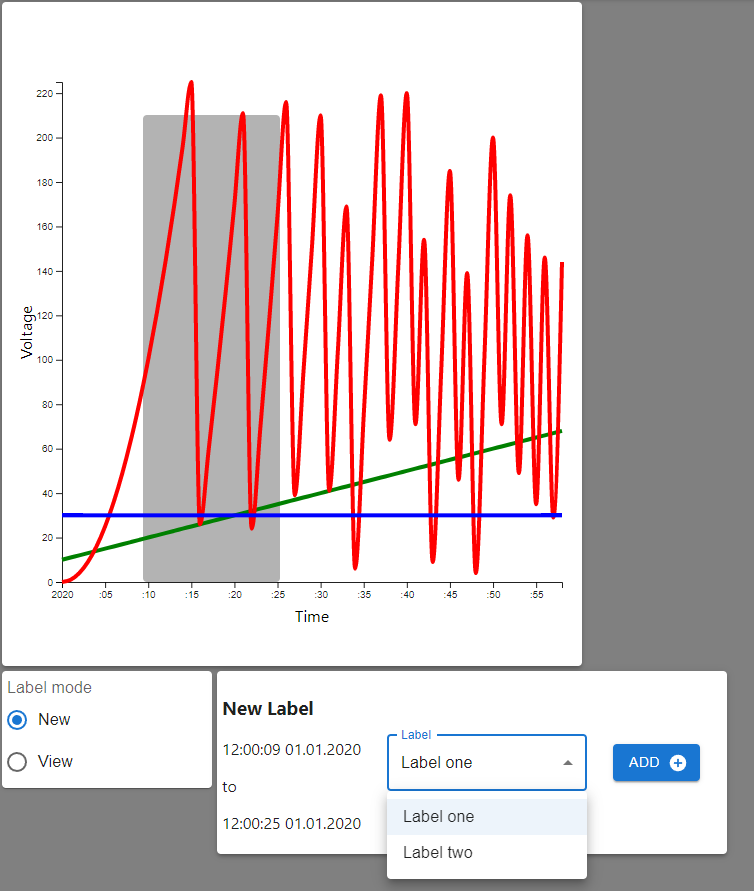
\includegraphics[width=1.0\textwidth]{gfx/newLabel}
    \caption{Benutzerschnittstelle bei der Erstellung eines neuen Labels}
    \label{fig:add_label}
\end{figure}
Mit dem `ADD` Knopf wird das neue Label an die \ac{API} übermittelt und dort abgespeichert.
Alle vorhandenen Labels werden als farbige Balken auf die Graphen gezeichnet.
Jedem Label-Typ wird dazu von der \ac{API} eine eigene Farbe zugewiesen.
In Abbildung \ref{fig:view_label} sind zwei Labels ersichtlich.
Um mehr Informationen über die Labels zu erhalten, kann bei der `Label mode` Komponente auf der linken Seite von
`New` auf `View` gewechselt werden.
Wird nun ein Label angeklickt,
erscheinen einige Informationen über das Label sowie eine Möglichkeit dieses zu löschen.
Um danach erneut Labels zu erstellen, muss der Modus wieder auf `New` gewechselt werden.



\begin{figure}[H]
    \centering
    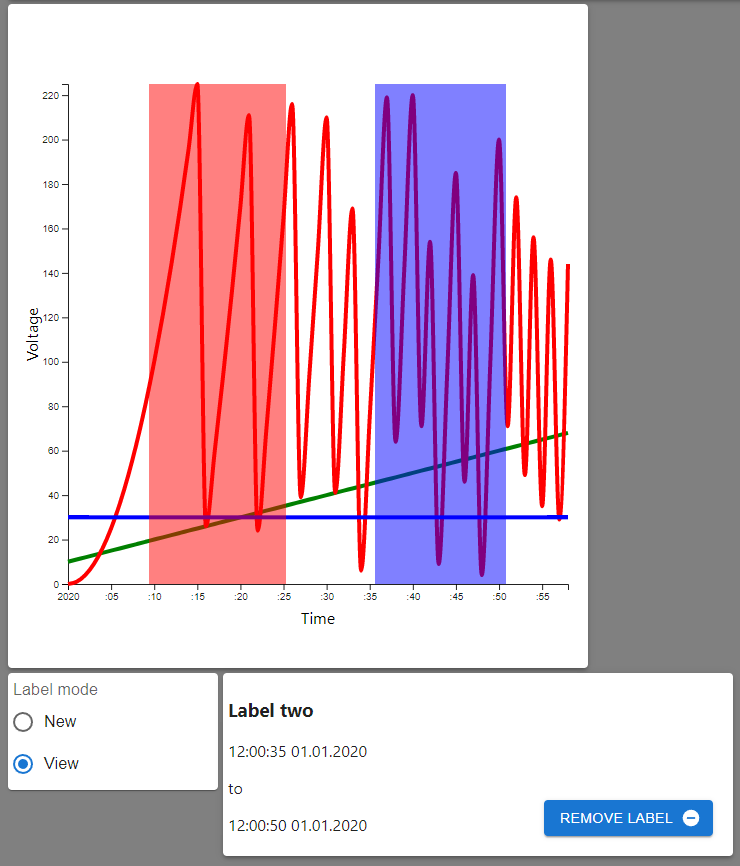
\includegraphics[width=1.0\textwidth]{gfx/viewLabel}
    \caption{Benutzerschnittstelle bei Inspektion eines bestehenden Labels}
    \label{fig:view_label}
\end{figure}

\subsubsection{API}
Die \ac{API} musste um einige Endpunkte erweitert werden:

\begin{verbatim}
    GET /label
\end{verbatim}
Gibt eine Liste aller verfügbaren Labels zurück.
Diese Liste ist einfachheitshalber nicht über die \ac{API} erweiterbar.
Die Einträge wurden direkt in die Datenbank eingetragen.
\begin{verbatim}
    GET /meters/{meter_id}/labels
\end{verbatim}
Gibt eine Liste aller Labels zurück, welche dem gewählten Zähler zugeordnet wurden.

\begin{verbatim}
    POST /meters/{meter_id}/labels
\end{verbatim}
Ermöglicht das Hinzufügen neuer Labels. Im Body müssen jeweils Angaben zur Start- und Endzeit
sowie gewähltem Label mitgeschickt werden.

\begin{verbatim}
    DELETE /labels/assignments/{assignment_id}
\end{verbatim}
Ermöglicht das Löschen einer zuvor erstellten Label-Zuordnung.

Die aufgeführten Endpunkte führen einfache Schreib- und Lesezugriffe auf die Datenbank aus.
Labels und Label-Zuweisungen sind in dieser Iteration neu zur Datenbank hinzugefügt worden.
Das vollständige Schema der Datenbank wird in Kapitel \ref{rel:db} beschrieben.


\subsection{\ac{TLS} Verschlüsselung}

Wie in der Aufgabenstellung (Anhang \ref{anhang:aufgabenstellung}) und vom Auftraggeber gewünscht, wurde
für das Übertragen der \ac{MQTT} Daten eine \ac{TLS} Verschlüsselung implementiert.

Mit \ac{TLS} können drei Sachen erreicht werden \parencite{what_is_tls}:

\begin{itemize}
    \item \texttt{Verschlüsselung}: Garantiert, dass gesendete Daten nicht von Dritten abgehört werden können.
    \item \texttt{Authentifizierung}: Versichert, dass die an der Kommunikation teilnehmenden Parteien, die sind für die sie sich ausgeben.
    \item \texttt{Integrität}: Verifiziert, dass gesendete Daten auf dem Sendeweg nicht durch Dritte geändert worden sind.
\end{itemize}

Erreicht wird dies durch SSL Zertifikate \parencite{what_is_ssl_certificate}. Diese sind auf dem Server
installiert und werden durch eine \ac{CA} ausgestellt \parencite{what_is_ca}.
Dadurch wird die Authentifizierung eines Servers sichergestellt.
Diese \ac{CA} ist eine vertrauenswürdige Stelle\footnote{
    Beispielsweise Letsencrypt \parencite{letsencrypt_2021}
}, welche sicherstellt, dass eine Domäne wirklich der Person gehört die das auch behauptet.
Um \ac{TLS} Verschlüsselung für die Entwicklung zu verwenden ist das jedoch nicht notwendig.
Hier kann mit sogenannten Self Signed Certificates gearbeitet werden \parencite{self_signed_cert}.
Der einzige Unterschied dabei ist, dass das Zertifikat nicht durch eine \ac{CA} signiert wird, sondern dass
dies selbst gemacht werden muss. In diesem Projekt wurde für die automatische Erstellung eines solchen
Zertifikates mkcert\footnote{https://github.com/FiloSottile/mkcert} verwendet.

Die Konfiguration des \ac{MQTT} Brokers kann basierend auf der Anleitung \parencite{mosquitto.conf_man_page_2021}
einfach vorgenommen werden:

\begin{verbatim}
cafile /rootCA.pem
certfile /localhost+4.pem
keyfile /localhost+4-key.pem
\end{verbatim}

Den Clients\footnote{
    In diesem fall ist das der \texttt{dataingress} die Daten verarbeitet und die verschiedenen
    Stromzähler welche die Daten senden.
} muss danach nur noch gesagt werden, welcher \ac{CA} sie vertrauen können.
In diesem Fall ist dies ein Self Signed Certificate namens \texttt{rootCA.pem}, das mittels
mkcert generiert wurde.

\subsection{Verifikation}

Um die korrekte Funktionalität der neu implementierten Anforderungen zu verifizieren, wurden
zwei neue End to End Tests implementiert. Diese verifizieren zum einen die Funktionalität der
Labelerstellung und zum anderen, ob die \ac{TLS} Verschlüsselung funktioniert (Abbildung \ref{fig:test-iteration-3}).

\begin{figure}[H]
    \centering
    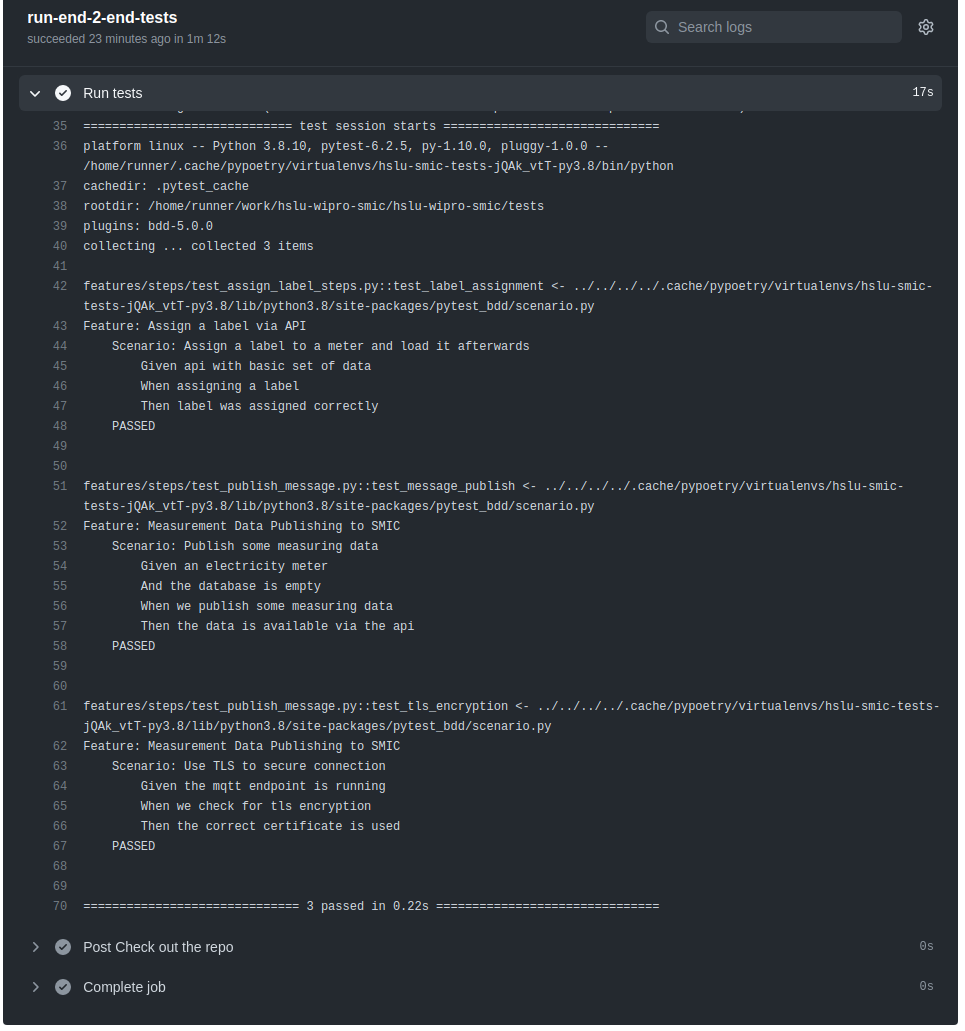
\includegraphics[width=1.0\textwidth]{gfx/testlog-iteration-2}
    \caption{
        Erweiterung der Tests um das Zuweisen von Labels und Testen der \ac{TLS} Verschlüsselung \parencite{randombenj_testlog_it_2_2021}
    }
    \label{fig:test-iteration-3}
\end{figure}

\subsection{Schwierigkeiten}
Die Python Library \texttt{paho}, welche für die \ac{MQTT} Kommunikation verwendet wird, so zu konfigurieren,
dass sie die \ac{TLS} Verschlüsselung unterstützt, stellte sich als Schwierigkeit heraus.
Nach einiger Recherche zeigte sich, dass \texttt{paho} ein unübliches \ac{TLS}
Verhalten aufweist \parencite{eclipse_paho_ssl_2019}.
Nachdem der Parameter \texttt{cert\_reqs=ssl.CERT\_NONE} gesetzt wurde, funktionierte
die \ac{TLS} Verschlüsselung dann auch.
Somit konnte zum Schluss der Iteration auch die letzte noch offene Anforderung erfüllt werden.